\documentclass[10pt]{beamer}

\usetheme{metropolis}
\usepackage{appendixnumberbeamer}

\usepackage{booktabs}
\usepackage[scale=2]{ccicons}
\usepackage{graphicx}
\usepackage{pgfplots}
\usepgfplotslibrary{dateplot}
\usepackage{caption}
\usepackage{subcaption}
\usepackage{xspace}
\usepackage{hyperref,xcolor}
\usepackage{textpos}
\usepackage{appendixnumberbeamer}
\usepackage{makeidx}
\usepackage{verbatim}
\definecolor{winered}{rgb}{0.5,0,0}
\newcommand{\themename}{\textbf{\textsc{metropolis}}\xspace}


\defbeamertemplate*{background canvas}{bg}
{%
	\color{white}\vrule width\paperwidth height\paperheight% added bg color
}





\title{Bhabha Tracking Efficiencies}
%\subtitle{A modern beamer theme}
\date{09.08.2019}
\author{Martin Sobotzik}
\institute{Johannes Gutenberg-Universit\"at Mainz}
% \titlegraphic{\hfill\includegraphics[height=1.5cm]{logo.pdf}}

\definecolor{darkblue}{rgb}{0,0,.5}
\hypersetup{pdftex=true, colorlinks=true, breaklinks=true, linkcolor=darkblue, menucolor=darkblue, pagecolor=darkblue, urlcolor=darkblue}


%citecolor={winered} %Gives errors when turned on
%allcolors={winered} %Gives errors when turned on

\begin{document}

\maketitle
%
\setbeamertemplate{frame footer}{}

%\section{Reproducing Plots}


\begin{frame}{Motivation}

\begin{itemize}	
	\item I am performing an analysis to estimate the tracking efficiency on phase 2 data
	\item The process I am considering is Bhabha events $\textrm{e}^+ \textrm{+e}^- \rightarrow \textrm{e}^+ \textrm{+e}^- $ 
	\item The definition of efficiency I am going to use is:

\end{itemize}
	\begin{equation*}
		\epsilon = \frac{\textrm{Number of Bhabha events with exactly 2 tracks}}{\textrm{Number of Bhabha events with 1 or more tracks}}
	\end{equation*}
	
	\begin{itemize}
		\item After selecting Bhabha events where at least one of the tracks was detected, one can look how many times the second one is found
		\item  This idea comes from some plots presented by Sam Cunliffe in previous  \href{https://confluence.desy.de/display/BI/ECL+Meetings?preview=/84320165/109161400/SCunliffe181123-ECL.pdf}{tracking and ECL} meetings.
	\end{itemize}





\end{frame}
	
	
\begin{frame}{Best Candidate Selection}
	
	\begin{textblock*}{\textwidth}(0cm,-4cm)
		\begin{center}	
			$\textrm{vpho} \rightarrow \textrm{ECL-Object(HclE)} + \textrm{ECL-Object(LclE)}$	
		\end{center}

	\end{textblock*}
	
	\begin{textblock*}{\textwidth}(0cm,-3.05cm)
		\scriptsize{		HcLE: particle with the higher cluster Energy; 	
		LclE: particle with the lower cluster Energy
}		
	\end{textblock*}

	
	
	
	\begin{textblock*}{1.2\textwidth}(-0.7cm,-2.8cm)
		

	
	
	\begin{itemize}
		
		\item $0.296706 < \theta_{\textrm{ECL Object}} < 2.61799 \rightarrow$ It has to hit the ECL
		\item Exactly two clusters with at least $3.5\,\textrm{GeV}$ per event
		\item $8\,\textrm{GeV} < \textrm{M}_{\textrm{vpho}} < 12\,\textrm{GeV}$
		\item $\textrm{nTracks} < 7$ 
		\item $\textrm{Total Energy in the ECL} < 15\,\textrm{GeV}$
						
		\end{itemize}

	\end{textblock*}


\begin{textblock*}{0.5\textwidth}(0cm,0.5cm)
	\includegraphics[width=4.5cm]{Plots/nCandMC}
\end{textblock*}


	
\begin{textblock*}{0.5\textwidth}(6cm,0.5cm)
	\includegraphics[width=4.5cm]{Plots/nCandData}
\end{textblock*}
	
	
\begin{textblock*}{0.5\textwidth}(1cm,0.5cm)
	\footnotesize
	\textcolor{red}{1 MC $\textrm{ee} \rightarrow \textrm{ee}$ File}
\end{textblock*}	
	
\begin{textblock*}{0.5\textwidth}(6.35cm,0.cm)
	\footnotesize
	\textcolor{blue}{Phase 2 data}
	
	\textcolor{blue}{r02608/all/mdst/sub00/*.root}
\end{textblock*}	

	
	
	
\end{frame}


\begin{frame}{Bhabha Event Selection}

	\begin{figure}
		\centering
		\includegraphics<1>[width=\textwidth]{Plots/b2b_2}
	\end{figure}
	
\end{frame}
	
	
\begin{frame}{Bhabha Event Selection (Phase 2 data)}
	
	\begin{textblock*}{0.5\textwidth}(0cm,-3cm)
		\centering
		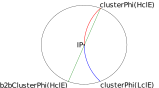
\includegraphics[width=4.5cm]{Plots/b2b_2}
	\end{textblock*}
	
	\begin{textblock*}{0.5\textwidth}(6cm,-3cm)
		\centering
		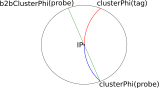
\includegraphics[width=4.5cm]{Plots/b2b_3}
	\end{textblock*}
	
	
	\begin{textblock*}{1\textwidth}(0cm,0.5cm)
		\centering
		\includegraphics[width=\textwidth]{Plots/Eff/b2b_Data.pdf}
	\end{textblock*}
	
	
	
	

		\begin{textblock*}{0.3\textwidth}(4.cm,0cm)
		\textcolor{blue}{Phase 2 data}		
		\textcolor{blue}{r02608}
	\end{textblock*}
	

	
	
	
	
	
\end{frame}
	
\begin{frame}{Bhabha Event Selection (MC)}	
	
		\begin{textblock*}{0.5\textwidth}(0cm,-3cm)
		\centering
		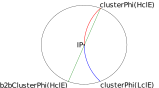
\includegraphics[width=4.5cm]{Plots/b2b_2}
	\end{textblock*}
	
	\begin{textblock*}{0.5\textwidth}(6cm,-3cm)
		\centering
		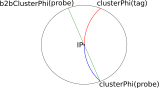
\includegraphics[width=4.5cm]{Plots/b2b_3}
	\end{textblock*}
	

		\begin{textblock*}{1\textwidth}(0cm,0.5cm)
		\centering
		\includegraphics[width=\textwidth]{Plots/Eff/b2b_MC.pdf}
	\end{textblock*}







	\begin{textblock*}{0.3\textwidth}(4.4cm,0cm)
		\textcolor{red}{MC: $\textrm{ee} \rightarrow \textrm{ee}$}
	\end{textblock*}





\end{frame}



\begin{frame}{More Events}
	\textcolor{red}{MC}:
	\begin{itemize}
	
		\item /belle/MC/release-02-00-01/DB00000411/MC11/prod00006731/
		s00/e1002/4S/r00000/3600520000/mdst/sub00
		\item $ 5272146$ candidates selected
	\end{itemize}
	\textcolor{blue}{Phase 2 data}:
	\begin{itemize}
		\item /ghi/fs01/belle2/bdata//Data/release-03-00-03/
		DB00000528/proc00000008/e0003/4S/r02*/all/mdst/sub00/*.root
		\item proc8
		\item $3669759$ candidates selected 
	\end{itemize}

\end{frame}









\begin{frame}{Compare MC And Phase 2 data Efficiency}
	\begin{figure}
		\centering
		\includegraphics[width=\textwidth]{Plots/Eff/TPMCData}
	\end{figure}

	\begin{textblock*}{0.3\textwidth}(-0.5cm,-5cm)
	$\textrm{e}^-$
\end{textblock*}
\begin{textblock*}{0.3\textwidth}(-0.5cm,-2cm)
	$\textrm{e}^+$
\end{textblock*}


\begin{textblock*}{0.3\textwidth}(1.65cm,-6.7cm)
	\textcolor{blue}{Phase 2 data}
\end{textblock*}


\begin{textblock*}{0.3\textwidth}(7.87cm,-6.7cm)
	\textcolor{red}{MC}
\end{textblock*}



\end{frame}

\begin{frame}{Theta And Phi Projection}
	\begin{figure}
		\centering
		\includegraphics[width=\textwidth]{Plots/Eff/MCDataEff}
	\end{figure}

	\begin{textblock*}{0.3\textwidth}(-0.5cm,-5cm)
		$\textrm{e}^-$
	\end{textblock*}
	\begin{textblock*}{0.3\textwidth}(-0.5cm,-2cm)
		$\textrm{e}^+$
	\end{textblock*}


	\begin{textblock*}{0.3\textwidth}(2.5cm,-6.7cm)
		$\Phi$
	\end{textblock*}


	\begin{textblock*}{0.3\textwidth}(7.87cm,-6.7cm)
	$\Theta$
\end{textblock*}


\begin{textblock*}{0.5\textwidth}(1cm,-5cm)
	\textcolor{blue}{Phase 2 data}
	
	\textcolor{red}{MC}
	
	
\end{textblock*}
	
\end{frame}

\begin{frame}{Theta And Phi Projection (Barrel Region Only)}
	\begin{figure}
		\centering
		\includegraphics[width=\textwidth]{Plots/Eff/PhiBarrel.pdf}
	\end{figure}
	
	
	\begin{textblock*}{0.3\textwidth}(-0.5cm,-5cm)
		$\textrm{e}^-$
	\end{textblock*}
	\begin{textblock*}{0.3\textwidth}(-0.5cm,-2cm)
		$\textrm{e}^+$
	\end{textblock*}
	
	
\begin{textblock*}{0.5\textwidth}(1cm,-5cm)
	\textcolor{blue}{Phase 2 data}
	
	\textcolor{red}{MC}
	
	
\end{textblock*}
	
		\begin{textblock*}{0.3\textwidth}(2.5cm,-6.7cm)
		$\Phi$
	\end{textblock*}
	
	
	\begin{textblock*}{0.3\textwidth}(7.87cm,-6.7cm)
		$\Theta$
	\end{textblock*}



\end{frame}

\begin{frame}{Ratio Between MC And Phase 2 Data}
	
	
	
	\begin{figure} 
	
	
	\centering
	\includegraphics[width=\textwidth]{Plots/Eff/Ratio}
\end{figure}
		\begin{textblock*}{0.3\textwidth}(-0.5cm,-5cm)
		$\textrm{e}^-$
	\end{textblock*}
	\begin{textblock*}{0.3\textwidth}(-0.5cm,-2cm)
		$\textrm{e}^+$
	\end{textblock*}
	
	
	\begin{textblock*}{0.3\textwidth}(2.5cm,-6.7cm)
		$\Phi$
	\end{textblock*}
	
	
	\begin{textblock*}{0.3\textwidth}(7.87cm,-6.7cm)
		$\Theta$
	\end{textblock*}
	
	
	
\end{frame}



\begin{frame}{Ratio Between MC And Phase 2 Data (Barrel Region Only)}
	\begin{figure}
		\centering
		\includegraphics[width=\textwidth]{Plots/Eff/BarrelRatio1.pdf}
	\end{figure}

		\begin{textblock*}{0.3\textwidth}(-0.5cm,-5cm)
	$\textrm{e}^-$
\end{textblock*}
\begin{textblock*}{0.3\textwidth}(-0.5cm,-2cm)
	$\textrm{e}^+$
\end{textblock*}


\begin{textblock*}{0.3\textwidth}(2.5cm,-6.7cm)
	$\Phi$
\end{textblock*}


\begin{textblock*}{0.3\textwidth}(7.87cm,-6.7cm)
	$\Theta$
\end{textblock*}




\end{frame}


\begin{frame}{Random}
	\begin{flushleft}

	Random means that in an event, I take a particle with a charge and check if the other particle has a track. (No a priori requirement on the charge of the tag particle)
	
			
\end{flushleft}
	\centering
	\includegraphics[width=\textwidth]{Additional/Random}
	
	
	\begin{textblock*}{0.3\textwidth}(0.8cm,-2.35cm)
		\scriptsize{Phase2 Data}
	\end{textblock*}
	
\begin{textblock*}{0.3\textwidth}(6.2cm,-2.35cm)
	\scriptsize{MC}
\end{textblock*}



	
\end{frame}







\begin{frame}{Random Ratio}
	\centering
	\includegraphics[width=\textwidth]{Additional/RandomRatio}
	
	
		\begin{textblock*}{0.3\textwidth}(0.8cm,-2.35cm)
		\scriptsize{\textcolor{white}{Ratio}}
	\end{textblock*}
	
	\begin{textblock*}{0.3\textwidth}(6.2cm,-2.35cm)
		\scriptsize{\textcolor{white}{Ratio Error}}
	\end{textblock*}
	
	
	
\end{frame}



\begin{frame}{Energy}
	This plot was created with a random event generator I wrote myself. It's just supposed to visualize the energy angle dependence of the Bhabha particles.
	\begin{figure}
		\centering
		\includegraphics[width=0.75\textwidth]{Plots/theta_lab.pdf}
	\end{figure}
\end{frame}


\begin{frame}{Momentum (MC)}
	\centering
	\includegraphics[width=0.9\textwidth]{Momentum/M_MC.pdf}

\begin{textblock*}{0.3\textwidth}(-1.6cm,-7.7cm)
	Random
\end{textblock*}

		\begin{textblock*}{0.3\textwidth}(-1.5cm,-5cm)
	$\textrm{e}^-$
\end{textblock*}
\begin{textblock*}{0.3\textwidth}(-1.5cm,-2cm)
	$\textrm{e}^+$
\end{textblock*}






\end{frame}

\begin{frame}{Momentum (Phase 2 Data)}
	\centering
	\includegraphics[width=0.9\textwidth]{Momentum/M_Data.pdf}
\begin{textblock*}{0.3\textwidth}(-1.6cm,-7.7cm)
	Random
\end{textblock*}

\begin{textblock*}{0.3\textwidth}(-1.5cm,-5cm)
	$\textrm{e}^-$
\end{textblock*}
\begin{textblock*}{0.3\textwidth}(-1.5cm,-2cm)
	$\textrm{e}^+$
\end{textblock*}	
	
	

\end{frame}










\begin{frame}{Momentum Random $\Phi$ Projection}
	\centering
	\includegraphics[width=0.8\textwidth]{Momentum/PMPhiRandom.pdf}


\begin{textblock*}{0.5\textwidth}(-2.45cm,-8cm)
	\small{
	\textcolor{blue}{Phase 2 data}
	
	\textcolor{red}{MC}
}
	
\end{textblock*}


\end{frame}


\begin{frame}{Momentum Random $\Theta$ Projection}
	\centering
	\includegraphics[width=0.8\textwidth]{Momentum/PMThetaRandom.pdf}
\end{frame}




\begin{frame}{Momentum $\textrm{e}^-$ $\Phi$ Projection}
	\centering
	\includegraphics[width=0.8\textwidth]{Momentum/PMPhiem.pdf}
\end{frame}


\begin{frame}{Momentum $\textrm{e}^-$ $\Theta$ Projection}
	\centering
	\includegraphics[width=0.8\textwidth]{Momentum/PMThetaem.pdf}
\end{frame}


\begin{frame}{Momentum $\textrm{e}^+$ $\Phi$ Projection}
	\centering
	\includegraphics[width=0.8\textwidth]{Momentum/PMPhiep.pdf}
\end{frame}


\begin{frame}{Momentum $\textrm{e}^+$ $\Theta$ Projection}
	\centering
	\includegraphics[width=0.8\textwidth]{Momentum/PMThetaep.pdf}
\end{frame}



%transsverse Momentum Hists.

\begin{frame}{Kinematic Transverse Momentum}
	This plot was also created with a  random event generator I wrote myself. Again, this only visualizes the transverse momentum of the Bhabha particles as a function of the $\theta$ angle.
	\begin{figure}
		\centering
		\includegraphics[width=0.75\textwidth]{Plots/ptTheta.pdf}
	\end{figure}
\end{frame}


\begin{frame}{Transverse Momentum (MC)}
	\centering
	\includegraphics[width=0.9\textwidth]{Momentum/transM_MC.pdf}
	\begin{textblock*}{0.3\textwidth}(-1.6cm,-7.7cm)
		Random
	\end{textblock*}
	
	\begin{textblock*}{0.3\textwidth}(-1.5cm,-5cm)
		$\textrm{e}^-$
	\end{textblock*}
	\begin{textblock*}{0.3\textwidth}(-1.5cm,-2cm)
		$\textrm{e}^+$
	\end{textblock*}
\end{frame}

\begin{frame}{Transverse Momentum (Phase 2 Data)}
	\centering
	\includegraphics[width=0.9\textwidth]{Momentum/transM_Data.pdf}
\begin{textblock*}{0.3\textwidth}(-1.6cm,-7.7cm)
	Random
\end{textblock*}

\begin{textblock*}{0.3\textwidth}(-1.5cm,-5cm)
	$\textrm{e}^-$
\end{textblock*}
\begin{textblock*}{0.3\textwidth}(-1.5cm,-2cm)
	$\textrm{e}^+$
\end{textblock*}

\end{frame}

\begin{frame}{Transverse Momentum Random $\Phi$ Projection}
	\centering
	\includegraphics[width=0.8\textwidth]{Momentum/PtMPhiRandom.pdf}
	\begin{textblock*}{0.5\textwidth}(-2.45cm,-8cm)
		\small{
			\textcolor{blue}{Phase 2 data}
			
			\textcolor{red}{MC}
		}
\end{textblock*}	
	
	
\end{frame}


\begin{frame}{Transverse Momentum Random $\Theta$ Projection}
	\centering
	\includegraphics[width=0.8\textwidth]{Momentum/PtMThetaRandom.pdf}
\end{frame}




\begin{frame}{Transverse Momentum $\textrm{e}^-$ $\Phi$ Projection}
	\centering
	\includegraphics[width=0.8\textwidth]{Momentum/PtMPhiem.pdf}
\end{frame}


\begin{frame}{Transverse Momentum $\textrm{e}^-$ $\Theta$ Projection}
	\centering
	\includegraphics[width=0.8\textwidth]{Momentum/PtMThetaem.pdf}
\end{frame}


\begin{frame}{Transverse Momentum $\textrm{e}^+$ $\Phi$ Projection}
	\centering
	\includegraphics[width=0.8\textwidth]{Momentum/PtMPhiep.pdf}
\end{frame}


\begin{frame}{Transverse Momentum $\textrm{e}^+$ $\Theta$ Projection}
	\centering
	\includegraphics[width=0.8\textwidth]{Momentum/PtMThetaep.pdf}
\end{frame}


\begin{frame}{Virtual Photon $\Phi$ (Single MC File)}
$\Phi$ angle of the virtual photon in a single MC file. Left before selection, right after selection.

\begin{figure}
	\centering
	\begin{minipage}{.5\textwidth}
		\centering
		\includegraphics[width=\textwidth]{gg/Phigg_BS}

	\end{minipage}%
	\begin{minipage}{.5\textwidth}
		\centering
		\includegraphics[width=\textwidth]{gg/Phigg_AS}

	\end{minipage}
\end{figure}
\end{frame}


\begin{frame}{Virtual Photon $\Phi$ And nTracks $\leq$ 1 (Single MC File)}
	$\Phi$ angle of the virtual photon in a single MC file. The number of tracks in each event has to be smaller than 2. Left before selection, right after selection.
	
	\begin{figure}
		\centering
		\begin{minipage}{.5\textwidth}
			\centering
			\includegraphics[width=\textwidth]{gg/Phigg_BS_nT1}
			
		\end{minipage}%
		\begin{minipage}{.5\textwidth}
			\centering
			\includegraphics[width=\textwidth]{gg/Phigg_AS_nT1}
			
		\end{minipage}
	\end{figure}



\end{frame}


\begin{frame}{Virtual Photon $\Theta$ (Single MC File)}
	$\Theta$ angle of the virtual photon in a single MC file. Left before selection, right after selection.
	
	\begin{figure}
		\centering
		\begin{minipage}{.5\textwidth}
			\centering
			\includegraphics[width=\textwidth]{gg/Thetagg_BS}
			
		\end{minipage}%
		\begin{minipage}{.5\textwidth}
			\centering
			\includegraphics[width=\textwidth]{gg/Thetagg_AS}
			
		\end{minipage}
	\end{figure}
\end{frame}


\begin{frame}{Virtual Photon $\Theta$ And nTracks $\leq$ 1 (Single MC File)}
	$\Theta$ angle of the virtual photon in a single MC file. The number of tracks in each event has to be smaller than 2. Left before selection, right after selection.
	
	\begin{figure}
		\centering
		\begin{minipage}{.5\textwidth}
			\centering
			\includegraphics[width=\textwidth]{gg/Thetagg_BS_nT1}
			
		\end{minipage}%
		\begin{minipage}{.5\textwidth}
			\centering
			\includegraphics[width=\textwidth]{gg/Thetagg_AS_nT1}
			
		\end{minipage}
	\end{figure}
	
	
	
\end{frame}




\begin{frame}{Virtual Photon $\Phi$ vs. $p$ (Single MC File)}
	$\Phi$ angle vs. the momentum of the virtual photon in a single MC file. Left before selection, right after selection.
	
	\begin{figure}
		\centering
		\begin{minipage}{.5\textwidth}
			\centering
			\includegraphics[width=\textwidth]{gg/PhiMgg_BS}
			
		\end{minipage}%
		\begin{minipage}{.5\textwidth}
			\centering
			\includegraphics[width=\textwidth]{gg/PhiMgg_AS}
			
		\end{minipage}
	\end{figure}
\end{frame}


\begin{frame}{Virtual Photon $\Phi$ vs. $p$ And nTracks $\leq$ 1 (Single MC File)}
	$\Phi$ angle vs. the momentum of the virtual photon in a single MC file. The number of tracks in each event has to be smaller than 2. Left before selection, right after selection.
	
	\begin{figure}
		\centering
		\begin{minipage}{.5\textwidth}
			\centering
			\includegraphics[width=\textwidth]{gg/PhiMgg_BS_nT1}
			
		\end{minipage}%
		\begin{minipage}{.5\textwidth}
			\centering
			\includegraphics[width=\textwidth]{gg/PhiMgg_AS_nT1}
			
		\end{minipage}
	\end{figure}
	
	
	
\end{frame}


\begin{frame}{Virtual Photon $\Theta$ vs. $p$ (Single MC File)}
	$\Theta$ angle vs. the momentum of the virtual photon in a single MC file. Left before selection, right after selection.
	
	\begin{figure}
		\centering
		\begin{minipage}{.5\textwidth}
			\centering
			\includegraphics[width=\textwidth]{gg/ThetaMgg_BS}
			
		\end{minipage}%
		\begin{minipage}{.5\textwidth}
			\centering
			\includegraphics[width=\textwidth]{gg/ThetaMgg_AS}
			
		\end{minipage}
	\end{figure}
\end{frame}


\begin{frame}{Virtual Photon $\Theta$ vs. $p$ And nTracks $\leq$ 1 (Single MC File)}
	$\Theta$ angle vs. the momentum of the virtual photon in a single MC file. The number of tracks in each event has to be smaller than 2. Left before selection, right after selection.
	
	\begin{figure}
		\centering
		\begin{minipage}{.5\textwidth}
			\centering
			\includegraphics[width=\textwidth]{gg/ThetaMgg_BS_nT1}
			
		\end{minipage}%
		\begin{minipage}{.5\textwidth}
			\centering
			\includegraphics[width=\textwidth]{gg/ThetaMgg_AS_nT1}
			
		\end{minipage}
	\end{figure}
	
	
	
\end{frame}




%Data



\begin{frame}{Virtual Photon $\Phi$ (Single Phase 2 File)}
	$\Phi$ angle of the virtual photon in a single Phase 2 file. Left before selection, right after selection.
	
	\begin{figure}
		\centering
		\begin{minipage}{.5\textwidth}
			\centering
			\includegraphics[width=\textwidth]{gg/data/Phigg_BS}
			
		\end{minipage}%
		\begin{minipage}{.5\textwidth}
			\centering
			\includegraphics[width=\textwidth]{gg/data/Phigg_AS}
			
		\end{minipage}
	\end{figure}
\end{frame}


\begin{frame}{Virtual Photon $\Phi$ And nTracks $\leq$ 1 (Single Phase 2 File)}
	$\Phi$ angle of the virtual photon in a single Phase 2 file. The number of tracks in each event has to be smaller than 2. Left before selection, right after selection.
	
	\begin{figure}
		\centering
		\begin{minipage}{.5\textwidth}
			\centering
			\includegraphics[width=\textwidth]{gg/data/Phigg_BS_nT1}
			
		\end{minipage}%
		\begin{minipage}{.5\textwidth}
			\centering
			\includegraphics[width=\textwidth]{gg/data/Phigg_AS_nT1}
			
		\end{minipage}
	\end{figure}
	
	
	
\end{frame}


\begin{frame}{Virtual Photon $\Theta$ (Single Phase 2 File)}
	$\Theta$ angle of the virtual photon in a single Phase 2 file. Left before selection, right after selection.
	
	\begin{figure}
		\centering
		\begin{minipage}{.5\textwidth}
			\centering
			\includegraphics[width=\textwidth]{gg/data/Thetagg_BS}
			
		\end{minipage}%
		\begin{minipage}{.5\textwidth}
			\centering
			\includegraphics[width=\textwidth]{gg/data/Thetagg_AS}
			
		\end{minipage}
	\end{figure}
\end{frame}


\begin{frame}{Virtual Photon $\Theta$ And nTracks $\leq$ 1 (Single Phase 2 File)}
	$\Theta$ angle of the virtual photon in a single MC file. The number of tracks in each event has to be smaller than 2. Left before selection, right after selection.
	
	\begin{figure}
		\centering
		\begin{minipage}{.5\textwidth}
			\centering
			\includegraphics[width=\textwidth]{gg/data/Thetagg_BS_nT1}
			
		\end{minipage}%
		\begin{minipage}{.5\textwidth}
			\centering
			\includegraphics[width=\textwidth]{gg/data/Thetagg_AS_nT1}
			
		\end{minipage}
	\end{figure}
	
	
	
\end{frame}












\begin{frame}{Virtual Photon $\Phi$ vs. $p$ (Single Phase 2 File)}
	$\Phi$ angle vs. the momentum of the virtual photon in a single Phase 2 file. Left before selection, right after selection.
	
	\begin{figure}
		\centering
		\begin{minipage}{.5\textwidth}
			\centering
			\includegraphics[width=\textwidth]{gg/data/PhiMgg_BS}
			
		\end{minipage}%
		\begin{minipage}{.5\textwidth}
			\centering
			\includegraphics[width=\textwidth]{gg/data/PhiMgg_AS}
			
		\end{minipage}
	\end{figure}
\end{frame}


\begin{frame}{Virtual Photon $\Phi$ vs. $p$ And nTracks $\leq$ 1 (Single Phase 2 File)}
	$\Phi$ angle vs. the momentum of the virtual photon in a single Phase 2 file. The number of tracks in each event has to be smaller than 2. Left before selection, right after selection.
	
	\begin{figure}
		\centering
		\begin{minipage}{.5\textwidth}
			\centering
			\includegraphics[width=\textwidth]{gg/data/PhiMgg_BS_nT1}
			
		\end{minipage}%
		\begin{minipage}{.5\textwidth}
			\centering
			\includegraphics[width=\textwidth]{gg/data/PhiMgg_AS_nT1}
			
		\end{minipage}
	\end{figure}
	
	
	
\end{frame}


\begin{frame}{Virtual Photon $\Theta$ vs. $p$ (Single Phase 2 File)}
	$\Theta$ angle vs. the momentum of the virtual photon in a single Phase 2 file. Left before selection, right after selection.
	
	\begin{figure}
		\centering
		\begin{minipage}{.5\textwidth}
			\centering
			\includegraphics[width=\textwidth]{gg/data/ThetaMgg_BS}
			
		\end{minipage}%
		\begin{minipage}{.5\textwidth}
			\centering
			\includegraphics[width=\textwidth]{gg/data/ThetaMgg_AS}
			
		\end{minipage}
	\end{figure}
\end{frame}


\begin{frame}{Virtual Photon $\Theta$ vs. $p$ And nTracks $\leq$ 1 (Single Phase 2 File)}
	$\Theta$ angle vs. the momentum of the virtual photon in a single Phase 2 file. The number of tracks in each event has to be smaller than 2. Left before selection, right after selection.
	
	\begin{figure}
		\centering
		\begin{minipage}{.5\textwidth}
			\centering
			\includegraphics[width=\textwidth]{gg/data/ThetaMgg_BS_nT1}
			
		\end{minipage}%
		\begin{minipage}{.5\textwidth}
			\centering
			\includegraphics[width=\textwidth]{gg/data/ThetaMgg_AS_nT1}
			
		\end{minipage}
	\end{figure}
	
	
	
\end{frame}










\begin{comment}

\begin{frame}{Summary}

	\begin{itemize}
		\item A first measurement of the tracking efficiency using the "b2b method" was presented (evaluated on a subsample of phase 2 data) 
		\item In the barrel region efficiency on data is slightly lower than on MC
		\item When including also the end cap regions the behavior of $\textrm{e}^+$ is not fully understood
		\item Further studies on the forward and backward region only are ongoing
	\end{itemize}


\end{frame}

	content...
\end{comment}


\section{Backup}
\appendix
\begin{frame}{ECL-Object}
	\begin{textblock*}{\textwidth}(0cm,-4cm)
		
		\begin{itemize}
			
			\item To have a complete list of objects with an ECL cluster associated, one needs to "mix" two different lists, one of gammas and one of electrons
			
		\end{itemize}
		
	\end{textblock*}
	\begin{textblock*}{\textwidth}(0cm,-2.9cm)
		
		
		\begin{figure}
			\includegraphics[width=10.5cm]{Plots/newSc}
		\end{figure}
		
	\end{textblock*}
	
	
	\begin{textblock*}{\textwidth}(0cm,-0.3cm)
		
		
		\begin{itemize}
			\item The electron list does not require a ECL cluster$\rightarrow$ problem solved with the cut on clusterE
			\item The framework does not allow to mix lists of different types $\rightarrow$ problem solved with the "trick" of two intermediate virtual photons
			\item The ranking is a way for me to have the order of the daughters' under control
			\item The Bhabha candidates are finally reconstructed starting from 2 ECLobjects
		\end{itemize}
	\end{textblock*}
\end{frame}










\begin{frame}{Theta And Phi Projection (Barrel Region Only)}
	\begin{figure}
		\centering
		\includegraphics[width=\textwidth]{Plots/Eff/PhiBarrel1.pdf}
	\end{figure}
	
	
	\begin{textblock*}{0.3\textwidth}(-0.5cm,-5cm)
		$\textrm{e}^-$
	\end{textblock*}
	\begin{textblock*}{0.3\textwidth}(-0.5cm,-2cm)
		$\textrm{e}^+$
	\end{textblock*}
	
	
	\begin{textblock*}{0.5\textwidth}(1cm,-0.2cm)
		\textcolor{blue}{Phase 2 data}
		
		\textcolor{red}{MC}
		
		
	\end{textblock*}
	
	\begin{textblock*}{0.3\textwidth}(2.5cm,-6.7cm)
		$\Phi$
	\end{textblock*}
	
	
	\begin{textblock*}{0.3\textwidth}(7.87cm,-6.7cm)
		$\Theta$
	\end{textblock*}
	
	
	
\end{frame}












\begin{frame}{Ratio between MC And Phase 2 data (Barrel Region Only)}
	\begin{figure}
		\centering
		\includegraphics[width=0.7\textwidth]{Plots/Eff/Ratio2d.pdf}
		
	\end{figure}
\end{frame}





\begin{frame}{Electron Efficiency (MC)}
	
	\begin{figure}
		\centering
		\includegraphics[width=\textwidth]{Plots/Eff/TPemEff}
	\end{figure}
	
\end{frame}

\begin{frame}{Positron Efficiency (MC)}
	
	\begin{figure}
		\centering
		\includegraphics[width=\textwidth]{Plots/Eff/TPepEff}
	\end{figure}
	
\end{frame}


\begin{frame}{Electron Efficiency (Phase 2 data)}
	
	\begin{figure}
		\centering
		\includegraphics[width=\textwidth]{Plots/Eff/TPemEff_Data}
	\end{figure}
	
\end{frame}

\begin{frame}{Positron Efficiency (Phase 2 data)}
	
	\begin{figure}
		\centering
		\includegraphics[width=\textwidth]{Plots/Eff/TPepEff_Data}
	\end{figure}
	
\end{frame}








\begin{frame}{Electron $\Phi$ Projection (Phase 2 data)}
	\centering
	\includegraphics[width=\textwidth]{Plots/Eff/emPhiPro_Data}
\end{frame}

\begin{frame}{Positron $\Phi$ Projection (Phase 2 data)}
	\centering
	\includegraphics[width=\textwidth]{Plots/Eff/epPhiPro_Data}
\end{frame}


\begin{frame}{Electron $\Theta$ Projection (Phase 2 data)}
	\centering
	\includegraphics[width=\textwidth]{Plots/Eff/emThetaPro_Data}
\end{frame}

\begin{frame}{Positron $\Theta$ Projection (Phase 2 data)}
	\centering
	\includegraphics[width=\textwidth]{Plots/Eff/epThetaPro_Data}
\end{frame}

\begin{frame}{Electron $\Phi$ Projection (MC)}
	\centering
	\includegraphics[width=\textwidth]{Plots/Eff/emPhiPro}
\end{frame}

\begin{frame}{Positron $\Phi$ Projection (MC)}
	\centering
	\includegraphics[width=\textwidth]{Plots/Eff/epPhiPro}
\end{frame}


\begin{frame}{Electron $\Theta$ Projection (MC)}
	\centering
	\includegraphics[width=\textwidth]{Plots/Eff/emThetaPro}
\end{frame}

\begin{frame}{Positron $\Theta$ Projection (MC)}
	\centering
	\includegraphics[width=\textwidth]{Plots/Eff/epThetaPro}
\end{frame}

\begin{frame}{Random $\Phi$ (Data)}
	\centering
	\includegraphics[width=\textwidth]{Additional/RandomPhi_Data}
\end{frame}

\begin{frame}{Random $\Theta$ (Data)}
	\centering
	\includegraphics[width=\textwidth]{Additional/RandomTheta_Data}
\end{frame}

\begin{frame}{Random $\Theta \Phi$ (Data)}
	\centering
	\includegraphics[width=\textwidth]{Additional/RandomTP_Data}
\end{frame}

\begin{frame}{Random $\Phi$ (MC)}
	\centering
	\includegraphics[width=\textwidth]{Additional/RandomPhi_MC}
\end{frame}

\begin{frame}{Random $\Theta$ (MC)}
	\centering
	\includegraphics[width=\textwidth]{Additional/RandomTheta_MC}
\end{frame}

\begin{frame}{Random $\Theta \Phi$ (MC)}
	\centering
	\includegraphics[width=\textwidth]{Additional/RandomTP_MC}
\end{frame}


\begin{frame}{Random Ratio}
	\centering
	\includegraphics[width=\textwidth]{Additional/RandomRatio}
\end{frame}







%%%%%%%%%%%%%%%%%%%%%%%%%%%%%%%%%%%%%%%%%%%%%%%%%%%%%%%%%%%%%%%%%%%%



\begin{frame}{Momentum Random $\Phi$ (MC)}
	\centering
	\includegraphics[width=\textwidth]{Momentum/MPhiRandom_MC}
\end{frame}


\begin{frame}{Momentum Random $\Theta$ (MC)}
	\centering
	\includegraphics[width=\textwidth]{Momentum/MThetaRandom_MC}
\end{frame}
\begin{frame}{Momentum $\textrm{e}^-$ $\Phi$ (MC)}
	\centering
	\includegraphics[width=\textwidth]{Momentum/MPhiem_MC}
\end{frame}


\begin{frame}{Momentum $\textrm{e}^-$ $\Theta$ (MC)}
	\centering
	\includegraphics[width=\textwidth]{Momentum/MThetaem_MC}
\end{frame}

\begin{frame}{Momentum $\textrm{e}^+$ $\Phi$ (MC)}
	\centering
	\includegraphics[width=\textwidth]{Momentum/MPhiep_MC}
\end{frame}


\begin{frame}{Momentum $\textrm{e}^+$ $\Theta$ (MC)}
	\centering
	\includegraphics[width=\textwidth]{Momentum/MThetaep_MC}
\end{frame}









\begin{frame}{Momentum Random $\Phi$ (Data)}
	\centering
	\includegraphics[width=\textwidth]{Momentum/MPhiRandom_Data}
\end{frame}


\begin{frame}{Momentum Random $\Theta$ (Data)}
	\centering
	\includegraphics[width=\textwidth]{Momentum/MThetaRandom_Data}
\end{frame}
\begin{frame}{Momentum $\textrm{e}^-$ $\Phi$ (Data)}
	\centering
	\includegraphics[width=\textwidth]{Momentum/MPhiem_Data}
\end{frame}


\begin{frame}{Momentum $\textrm{e}^-$ $\Theta$ (Data)}
	\centering
	\includegraphics[width=\textwidth]{Momentum/MThetaem_Data}
\end{frame}

\begin{frame}{Momentum $\textrm{e}^+$ $\Phi$ (Data)}
	\centering
	\includegraphics[width=\textwidth]{Momentum/MPhiep_Data}
\end{frame}


\begin{frame}{Momentum $\textrm{e}^+$ $\Theta$ (Data)}
	\centering
	\includegraphics[width=\textwidth]{Momentum/MThetaep_Data}
\end{frame}




%%%%%%%%%%%%%%%%%%%%%%%%%%%%%%%%%%%%%%%%%%%%%%%%%%%%%%

\begin{frame}{Transverse Momentum Random $\Phi$ (MC)}
	\centering
	\includegraphics[width=\textwidth]{Momentum/tMPhiRandom_MC}
\end{frame}


\begin{frame}{Transverse Momentum Random $\Theta$ (MC)}
	\centering
	\includegraphics[width=\textwidth]{Momentum/tMThetaRandom_MC}
\end{frame}
\begin{frame}{Transverse Momentum $\textrm{e}^-$ $\Phi$ (MC)}
	\centering
	\includegraphics[width=\textwidth]{Momentum/tMPhiem_MC}
\end{frame}


\begin{frame}{Transverse Momentum $\textrm{e}^-$ $\Theta$ (MC)}
	\centering
	\includegraphics[width=\textwidth]{Momentum/tMThetaem_MC}
\end{frame}

\begin{frame}{Transverse Momentum $\textrm{e}^+$ $\Phi$ (MC)}
	\centering
	\includegraphics[width=\textwidth]{Momentum/tMPhiep_MC}
\end{frame}


\begin{frame}{Transverse Momentum $\textrm{e}^+$ $\Theta$ (MC)}
	\centering
	\includegraphics[width=\textwidth]{Momentum/tMThetaep_MC}
\end{frame}


\begin{frame}{Transverse Momentum Random $\Phi$ (Data)}
	\centering
	\includegraphics[width=\textwidth]{Momentum/tMPhiRandom_Data}
\end{frame}


\begin{frame}{Transverse Momentum Random $\Theta$ (Data)}
	\centering
	\includegraphics[width=\textwidth]{Momentum/tMThetaRandom_Data}
\end{frame}
\begin{frame}{Transverse Momentum $\textrm{e}^-$ $\Phi$ (Data)}
	\centering
	\includegraphics[width=\textwidth]{Momentum/tMPhiem_Data}
\end{frame}


\begin{frame}{Transverse Momentum $\textrm{e}^-$ $\Theta$ (Data)}
	\centering
	\includegraphics[width=\textwidth]{Momentum/tMThetaem_Data}
\end{frame}

\begin{frame}{Transverse Momentum $\textrm{e}^+$ $\Phi$ (Data)}
	\centering
	\includegraphics[width=\textwidth]{Momentum/tMPhiep_Data}
\end{frame}


\begin{frame}{Transverse Momentum $\textrm{e}^+$ $\Theta$ (Data)}
	\centering
	\includegraphics[width=\textwidth]{Momentum/tMThetaep_Data}
\end{frame}




\end{document}
